% This is "sig-alternate.tex" V2.1 April 2013
% This file should be compiled with V2.5 of "sig-alternate.cls" May 2012
%
% This example file demonstrates the use of the 'sig-alternate.cls'
% V2.5 LaTeX2e document class file. It is for those submitting
% articles to ACM Conference Proceedings WHO DO NOT WISH TO
% STRICTLY ADHERE TO THE SIGS (PUBS-BOARD-ENDORSED) STYLE.
% The 'sig-alternate.cls' file will produce a similar-looking,
% albeit, 'tighter' paper resulting in, invariably, fewer pages.
%
% ----------------------------------------------------------------------------------------------------------------
% This .tex file (and associated .cls V2.5) produces:
%       1) The Permission Statement
%       2) The Conference (location) Info information
%       3) The Copyright Line with ACM data
%       4) NO page numbers
%
% as against the acm_proc_article-sp.cls file which
% DOES NOT produce 1) thru' 3) above.
%
% Using 'sig-alternate.cls' you have control, however, from within
% the source .tex file, over both the CopyrightYear
% (defaulted to 200X) and the ACM Copyright Data
% (defaulted to X-XXXXX-XX-X/XX/XX).
% e.g.
% \CopyrightYear{2007} will cause 2007 to appear in the copyright line.
% \crdata{0-12345-67-8/90/12} will cause 0-12345-67-8/90/12 to appear in the copyright line.
%
% ---------------------------------------------------------------------------------------------------------------
% This .tex source is an example which *does* use
% the .bib file (from which the .bbl file % is produced).
% REMEMBER HOWEVER: After having produced the .bbl file,
% and prior to final submission, you *NEED* to 'insert'
% your .bbl file into your source .tex file so as to provide
% ONE 'self-contained' source file.
%
% ================= IF YOU HAVE QUESTIONS =======================
% Questions regarding the SIGS styles, SIGS policies and
% procedures, Conferences etc. should be sent to
% Adrienne Griscti (griscti@acm.org)
%
% Technical questions _only_ to
% Gerald Murray (murray@hq.acm.org)
% ===============================================================
%
% For tracking purposes - this is V2.0 - May 2012

\documentclass{sig-alternate-05-2015}

\usepackage{subfloat}
\usepackage{subfig}
\usepackage{graphicx}

\begin{document}

% Copyright
%\setcopyright{acmcopyright}
%\setcopyright{acmlicensed}
%\setcopyright{rightsretained}
%\setcopyright{usgov}
%\setcopyright{usgovmixed}
%\setcopyright{cagov}
%\setcopyright{cagovmixed}


% DOI
%\doi{10.475/123_4}
%
%% ISBN
%\isbn{123-4567-24-567/08/06}
%
%%Conference
%\conferenceinfo{PLDI '13}{June 16--19, 2013, Seattle, WA, USA}
%
%\acmPrice{\$15.00}

%
% --- Author Metadata here ---
\conferenceinfo{IntSim}{2015, Augsburg}
%\CopyrightYear{2007} % Allows default copyright year (20XX) to be over-ridden - IF NEED BE.
%\crdata{0-12345-67-8/90/01}  % Allows default copyright data (0-89791-88-6/97/05) to be over-ridden - IF NEED BE.
% --- End of Author Metadata ---

\title{Come Fly With Me -- Perceive the World Through a Mosquito's Senses}
%
% You need the command \numberofauthors to handle the 'placement
% and alignment' of the authors beneath the title.
%
% For aesthetic reasons, we recommend 'three authors at a time'
% i.e. three 'name/affiliation blocks' be placed beneath the title.
%
% NOTE: You are NOT restricted in how many 'rows' of
% "name/affiliations" may appear. We just ask that you restrict
% the number of 'columns' to three.
%
% Because of the available 'opening page real-estate'
% we ask you to refrain from putting more than six authors
% (two rows with three columns) beneath the article title.
% More than six makes the first-page appear very cluttered indeed.
%
% Use the \alignauthor commands to handle the names
% and affiliations for an 'aesthetic maximum' of six authors.
% Add names, affiliations, addresses for
% the seventh etc. author(s) as the argument for the
% \additionalauthors command.
% These 'additional authors' will be output/set for you
% without further effort on your part as the last section in
% the body of your article BEFORE References or any Appendices.

\numberofauthors{1} %  in this sample file, there are a *total*
% of EIGHT authors. SIX appear on the 'first-page' (for formatting
% reasons) and the remaining two appear in the \additionalauthors section.
%
\author{
% You can go ahead and credit any number of authors here,
% e.g. one 'row of three' or two rows (consisting of one row of three
% and a second row of one, two or three).
%
% The command \alignauthor (no curly braces needed) should
% precede each author name, affiliation/snail-mail address and
% e-mail address. Additionally, tag each line of
% affiliation/address with \affaddr, and tag the
% e-mail address with \email.
%
% 1st. author
\alignauthor
Christopher Stifter\\
       \affaddr{University of Augsburg}\\
       \email{christopher.stifter@student.uni-augsburg.de}
       }
% There's nothing stopping you putting the seventh, eighth, etc.
% author on the opening page (as the 'third row') but we ask,
% for aesthetic reasons that you place these 'additional authors'
% in the \additional authors block, viz.
%\additionalauthors{Additional authors: John Smith (The Th{\o}rv{\"a}ld Group,
%email: {\texttt{jsmith@affiliation.org}}) and Julius P.~Kumquat
%(The Kumquat Consortium, email: {\texttt{jpkumquat@consortium.net}}).}
%\date{30 July 1999}
% Just remember to make sure that the TOTAL number of authors
% is the number that will appear on the first page PLUS the
% number that will appear in the \additionalauthors section.

\maketitle
\begin{abstract}
Mosquitoes are one of the deadliest (and most annoying) animal families in the world. They occur in a huge variety with different traits. In a lot of genera, the female mosquitoes suck blood from hosts for being able to reproduce. As a result, some are a major vector of infectious diseases. For tracking down blood sources mosquitoes are equipped with specialized senses. Within the scope of an interactive simulation, we want to present a simulation world to the user similar to how mosquitoes would perceive it, thus understanding the perception of the world by an alien life form. The user will be able to control the mosquito in first person view. The objective for the user is to find prey and suck blood using the available game mechanics, which represent the mosquito senses.
\end{abstract}

\begin{figure*}[bth!]
 %   \centering
\subfloat[The island from above.]{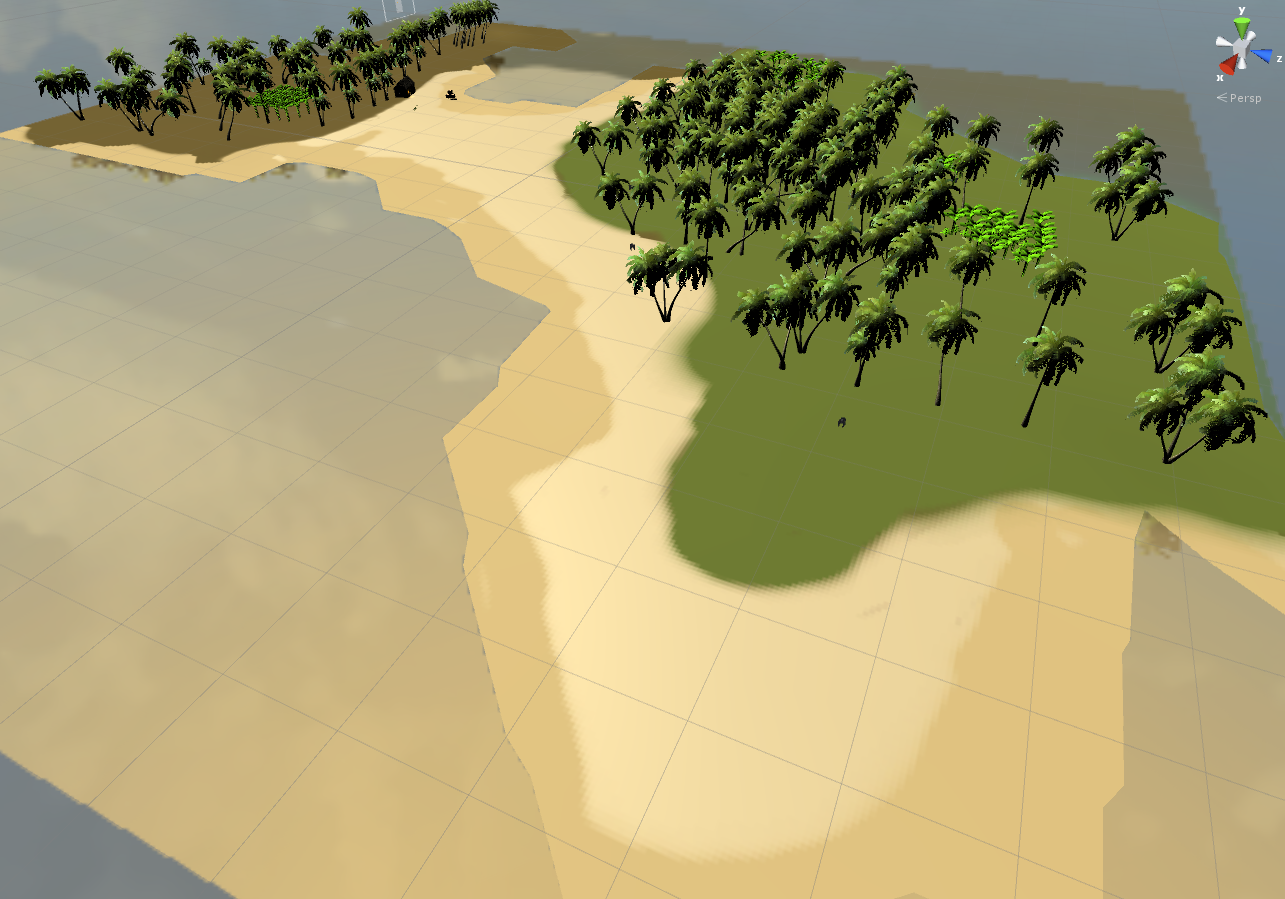
\includegraphics[width=0.5\textwidth, height=5.1cm]{Figures/island_topview.png}
\label{fig:islandabove}}
\subfloat[Zoomed in view on arbitrary part of the island.]{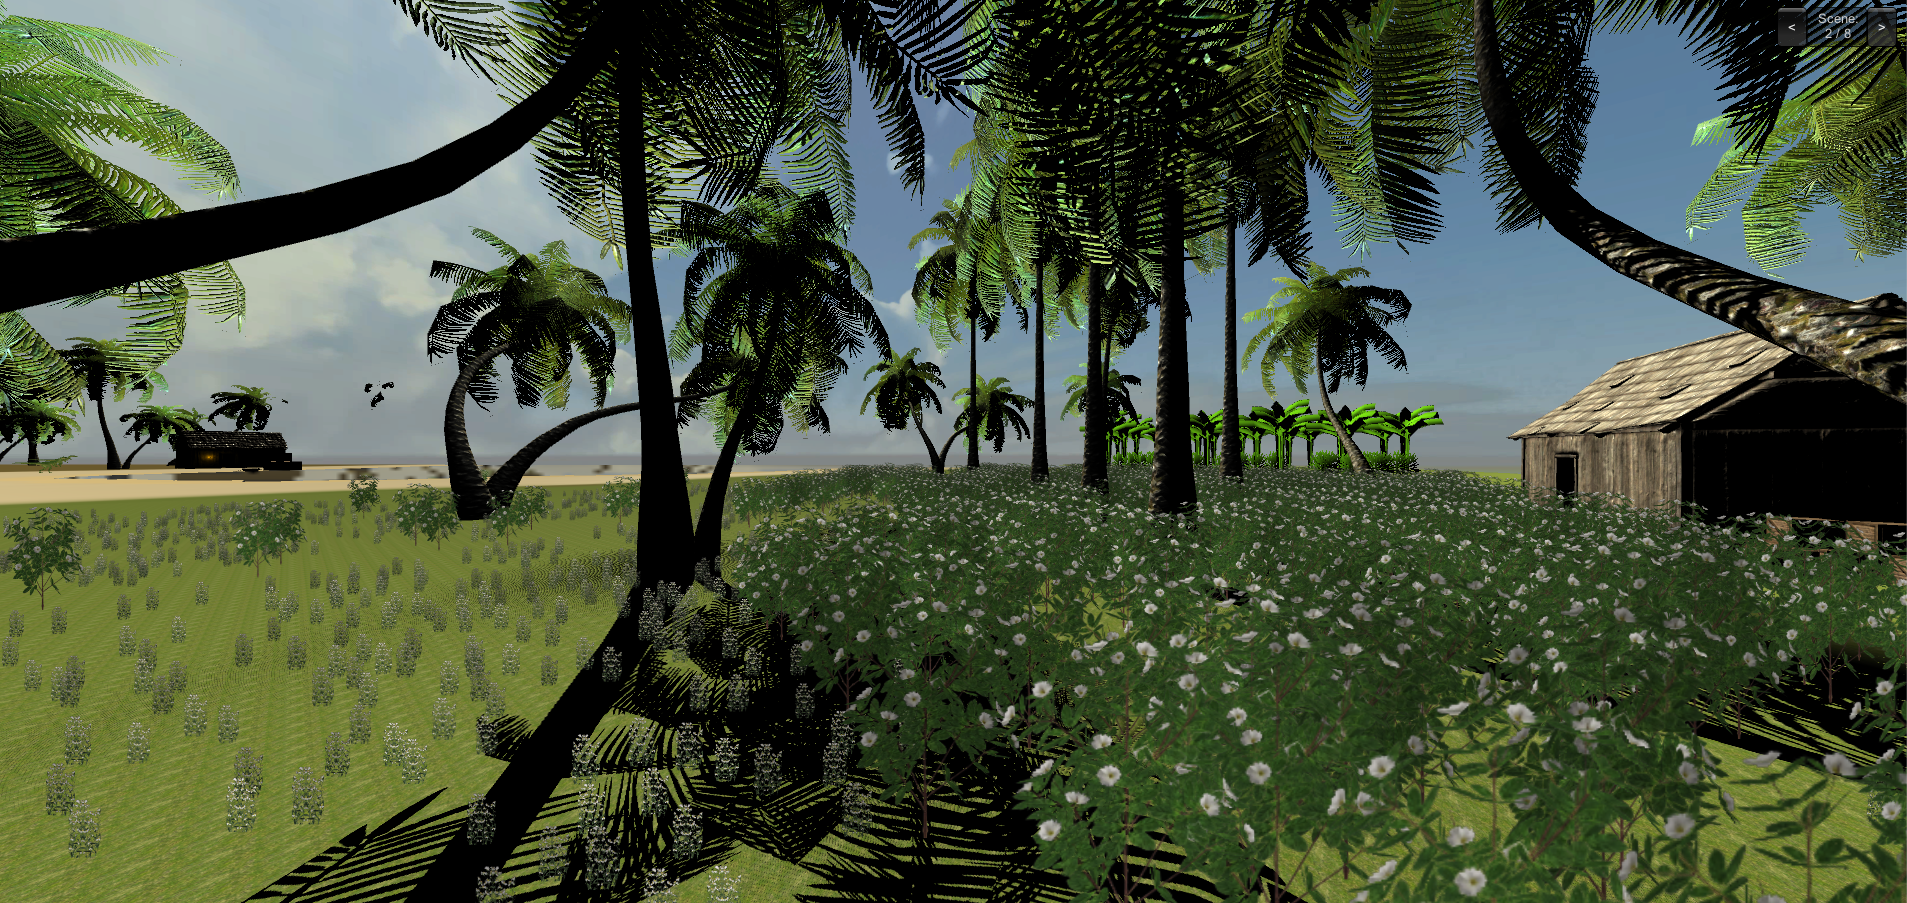
\includegraphics[width=0.5\textwidth, height=5.1cm]{Figures/island.png}
	\label{fig:island}}

\caption{The tropical island which serves as the simulation world. It consists of a rudimentary vegetation (mainly palms and banana trees), some solid objects (e.g. huts), and some animals.}
\label{fig:island_several}
\end{figure*}

\section{Introduction}
The word ``mosquito'' is Spanish for ``little fly''\cite{howstuff}. There have been over 2.700 species identified and described. Their distribution area is comprising almost the whole world (with the exception of Antarctica and some polar and sub-polar regions). The females of some species feed on blood. This is necessary for them to attain the ability lay eggs, because they need the proteins for their eggs. In passing from host to host it is possible for some species to transmit infectious, deadly diseases (e.g. malaria, yellow fever, dengue fever), if the mosquito bites a host. This means that additionally to the annoyance a mosquito represents, a real danger is added. In light of this, research on the behaviour of mosquitoes when hunting, on their reaction to environmental stimuli, on the features of their senses, and on deducing viable counter-measures from the gained data of these research areas becomes mandatory. Furthermore, the vastly different insect perception of the environment holds also great potential for technical applications.
In order to promote knowledge about this topic and to enable people to comprehend the influences on mosquitoes when searching for hosts, we developed an interactive simulation. This simulation will make it possible for the user to perceive the environment similar to the way a mosquito does. Through an appropriate mapping of the mosquito's senses, the user will be enabled to use these senses inside the simulation to track down blood sources.
In the remainder of this paper, we will first discuss similar work and efforts (cf. Section~\ref{sec:relatedwork}). In Section~\ref{sec:models}, we will describe what the simulation does and how the user can interact with it. In the subsequent Section~\ref{sec:projectreq} we will relate Section~\ref{sec:models} with the project requirements and how these requirements are addressed in the simulation. Finally, we conclude with ideas for future work and give a short summary in Section~\ref{sec:summary}.

\section{Related Work}
\label{sec:relatedwork}

An important feature of mosquitoes respectively of a lot of insects are their compound eyes. Compound eyes ``combine small eye volumes with a large field of view at the cost of comparatively low spatial resolution''~\cite{duparre2006}. Transferring the concept of compound eyes to technical systems has inspired the usage in micro-optics technology. For further details, see~\cite{duparre2006, duparre2004, voelkel2003, hamanaka1996}.
Furthermore, efforts to use these artificial compound eyes in robotics have been made (cf.~\cite{martin1994, lichtensteiger1999}). 

Simulations conveying different aspects of compound eyes to the user can be found in~\cite{giger, vorobyev1996, williams2007}.
Schenato et al.~\cite{schenato2001} presented a software testbed for simulating insect flight.

One possibility to avoid the spread of diseases through mosquitoes may be the usage of traps. Almeida et al.~\cite{almeida2010} simulated this approach with a multi-agent model, using a mosquito population, ``some mammals and objects found in urban environments'' and evaluated, if such an approach could control a mosquito population. 

An analysis of mosquito host-seeking behaviour within a simulation can be found in~\cite{iams2014}. Iams~\cite{cummins2012} measures and simulates the mosquito's motion and examines their flight stability and orientation.

In our simulation, we focus on the user experience and try to convey to the user how a mosquito perceives the environment.


\section{Models and Methods}
\label{sec:models}
In our interactive simulation, the user controls a female mosquito from first person view. Therefore, he can use representations of various mosquito senses to track down potential hosts. After landing, the user can initiate the process of blood sucking. During this process, he is exposed to the hosts counter measures. These counter measures are telegraphed to him through appropriate tells. In case the user manages to react to them in time, he has successfully fed on the host's blood---otherwise he dies. After having successfully fed two times, the user wins and the simulation starts all over on a higher difficulty level.


The simulation is set on a tropical island (cf. Figure~\ref{fig:island_several}), where mosquitoes are more common. This fits very nicely with the mosquito theme. The island consists of a wide beach, and two regions where grass and trees grow. The main floral assets used are different palms, banana trees, bushes, and flowers. Some solid objects like huts, crates, boats, fences, chairs, and benches are scattered throughout the island. The animal life is composed of gorillas (cf. Figure~\ref{fig:gorilla}) and velociraptor-like dinosaurs (cf. Figure~\ref{fig:dino}). Some of the animals freely roam the island, others are standing still.

\begin{figure}[ht!]
 %   \centering
\subfloat[The gorilla asset. ]{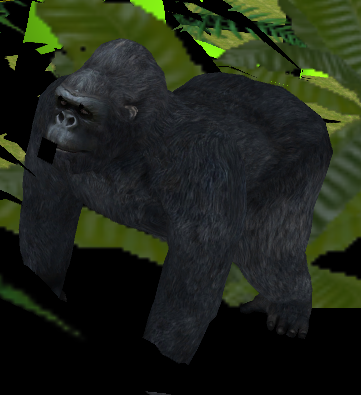
\includegraphics[width=0.235\textwidth, height=4.4cm]{Figures/gorilla.png}
\label{fig:gorilla}}
\subfloat[The dino asset.]{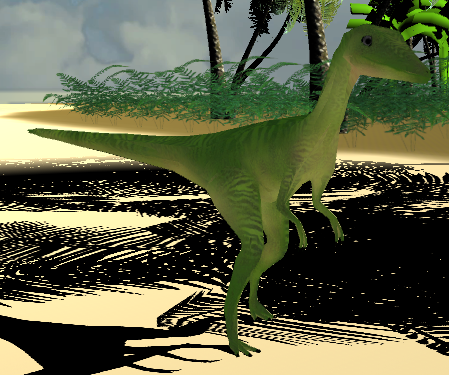
\includegraphics[width=0.235\textwidth, height=4.4cm]{Figures/dino.png}
	\label{fig:dino}}

\caption{The two used animal assets. Both may be moving in the simulation or stand still.}
\label{fig:animals}
\end{figure}

The GUI for the interactive simulation menu (cf. Figure~\ref{fig:gui}) is very simple. There are three buttons to interact with. The user can either start the simulation, view the tutorial, or quit the simulation. In the tutorial screen, the user can look up how his controls are configured (e.g. movement, landing on a host, initiate blood-sucking), what his objectives are, and can view some screenshots which serve as guidance regarding the game mechanics.

\begin{figure}[ht!]
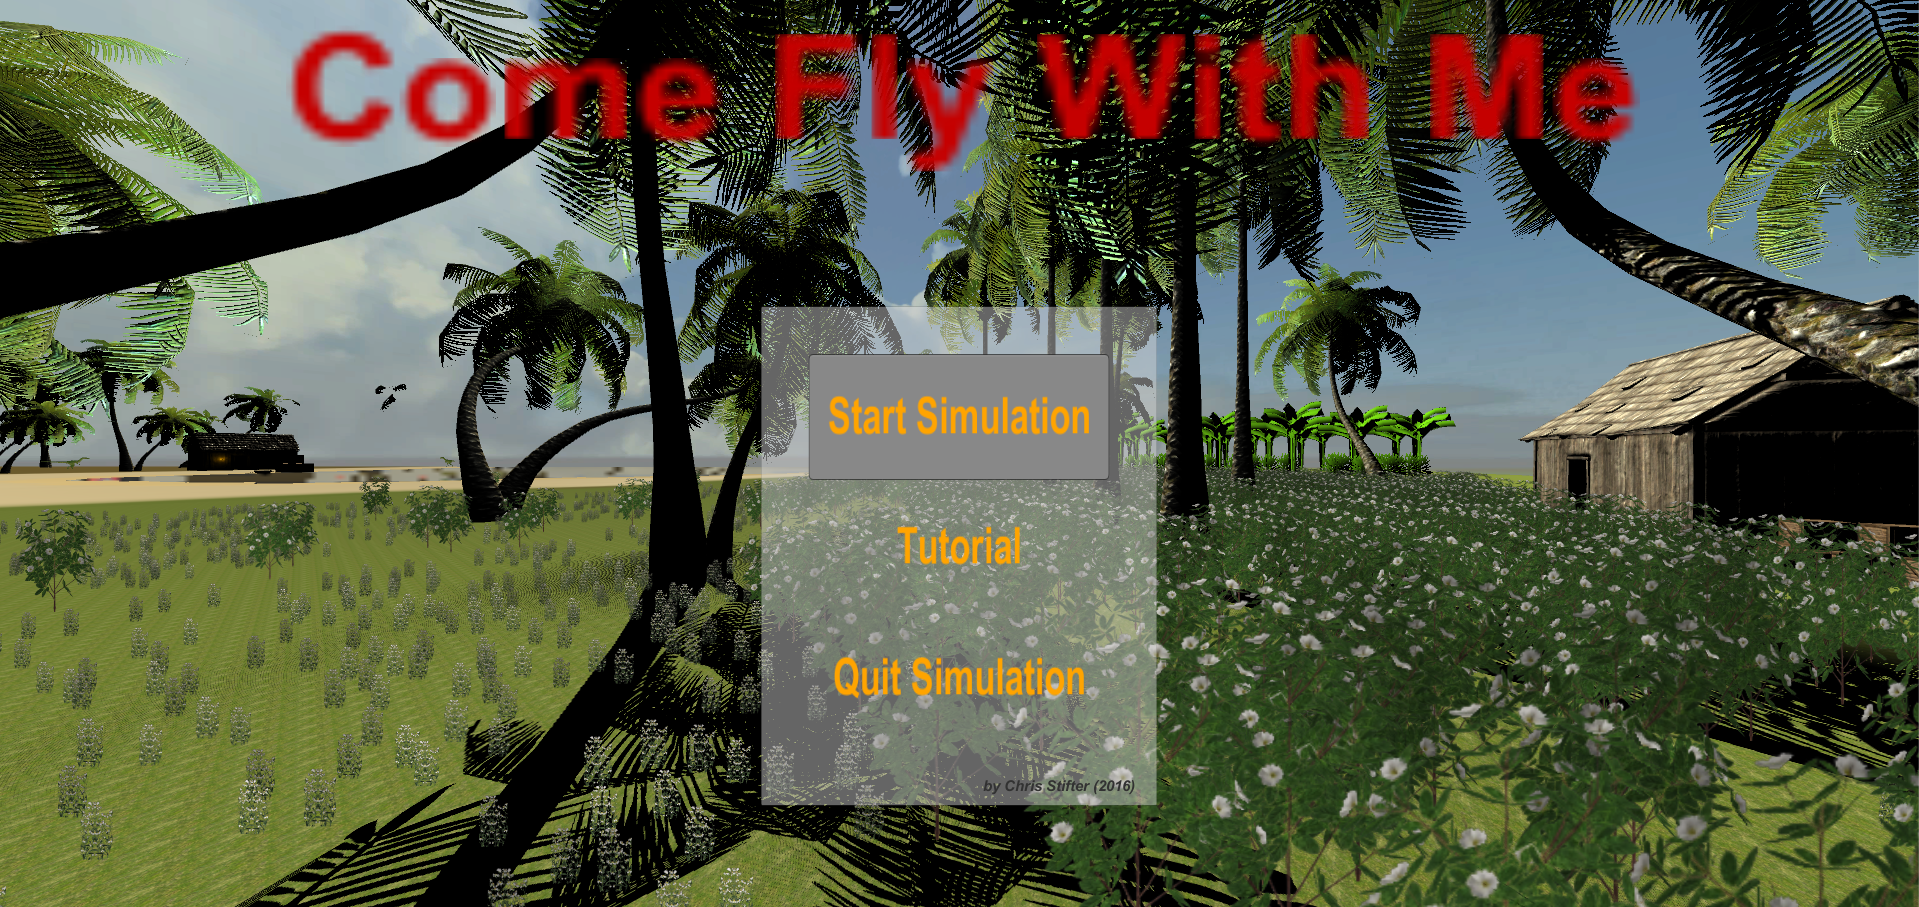
\includegraphics[width=0.47\textwidth]{Figures/gui.png}
\caption{The game menu. It shows the title of the simulation in a preliminary lettering and three buttons for starting the simulation, watching a tutorial, and ending the simulation.}
\label{fig:gui}
\end{figure}

\subsection{Representation of Mosquito Senses}
\label{sec:senses}
Female mosquitoes of blood-feeding mosquito species have highly optimised senses for searching hosts. The three important senses involved in localising prey are visual, chemical, and heat sensors. 

The interactive simulation is presented to the user with a far lower range of vision (cf. Figure~\ref{fig:vision}) compared to the viewing distance of humans. Furthermore, the spatial resolution is greatly reduced. Depending on whether the simulation is running on the first or second difficulty level the spatial resolution is either 39x22 (cf. Figure~\ref{fig:vision_highres}) or 33x18 (cf. Figure~\ref{fig:vision_lowres}). Additionally, the user experiences a soft screen shake from time to time. This emulates the susceptibility of the mosquito to wind impacts.


The second sense we have to address is the chemical sense, i.e. ``smelling''. Mosquitoes use the detection of \textit{carbon-dioxide}($CO_2$)---among other odours---to find potential hosts. We decided to map this sense to a visual representation. We use red globes (cf. Figure~\ref{fig:co2}) to represent carbon-dioxide. Every animal breathes these red globes, which are affected by wind, die after a certain time, and travel farther from their source (i.e. animal) than the user can see in the simulation. Moreover, the colour red is very distinct from the other colours in the simulation. This way, it is an object, which is easy to identify, and to follow. Additionally, if the mosquito moves through such an orb, its movement speed is increased for three seconds.

\begin{figure}[ht!]
 %   \centering
\subfloat[]{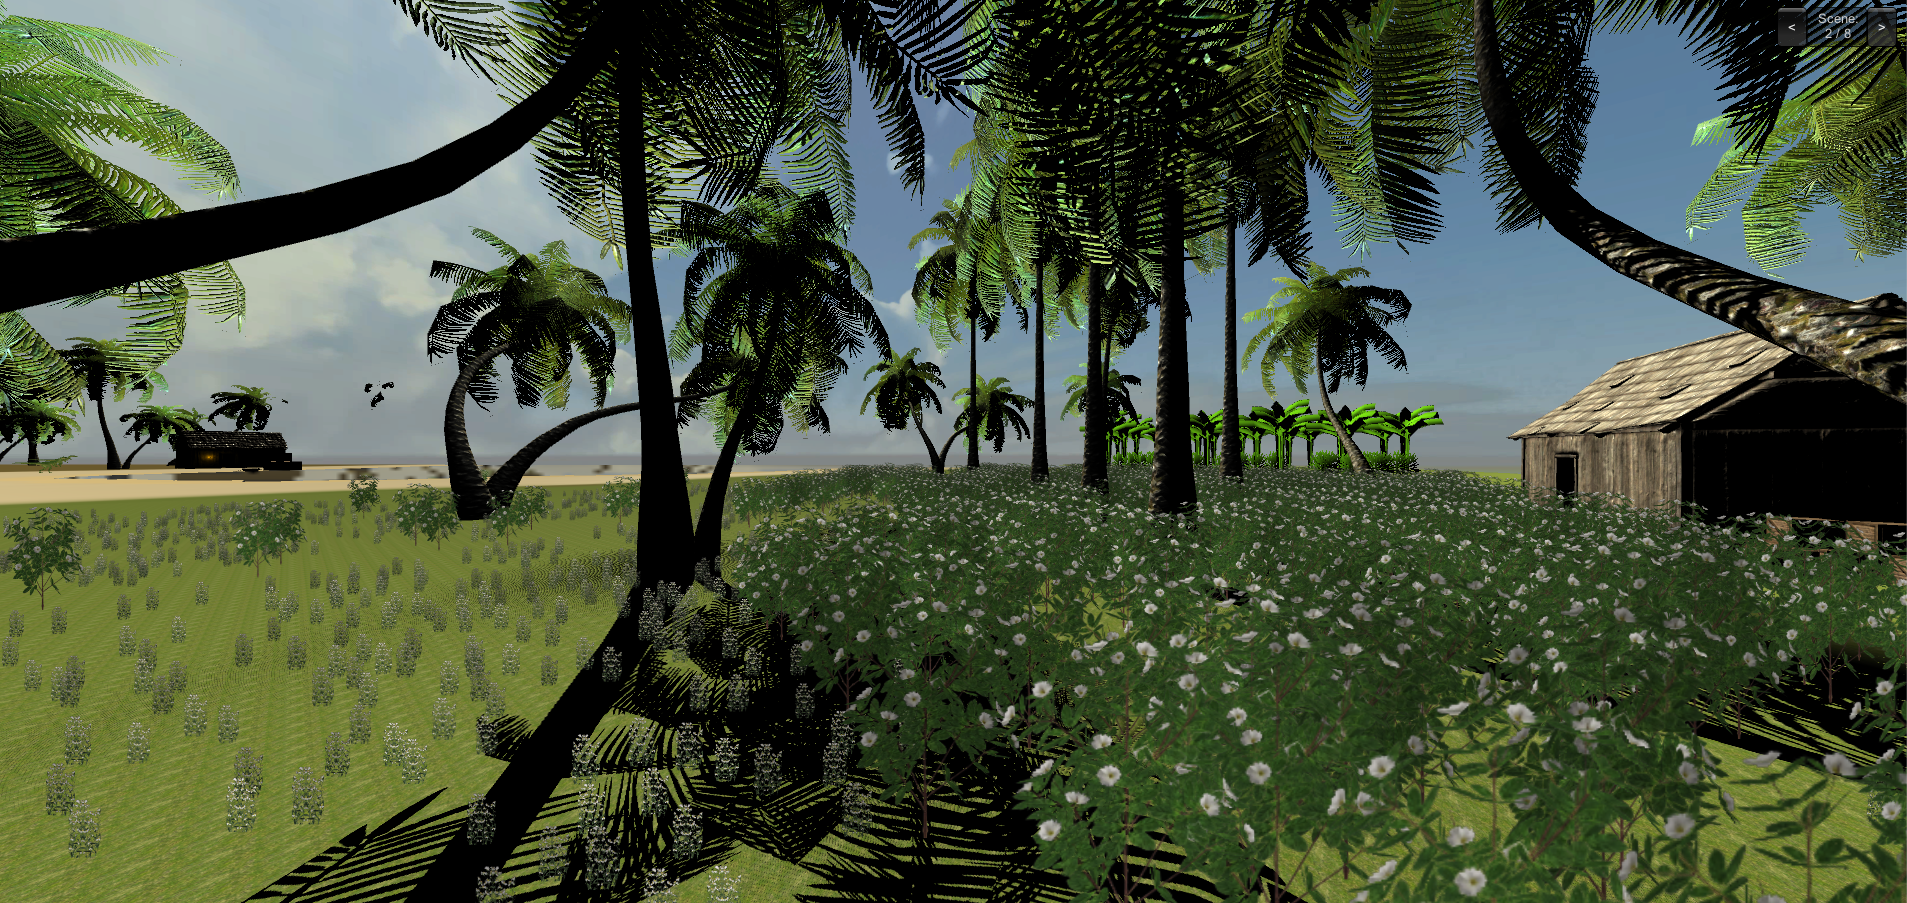
\includegraphics[width=0.235\textwidth]{Figures/island.png}
	\label{fig:vision_normal}}
\subfloat[]{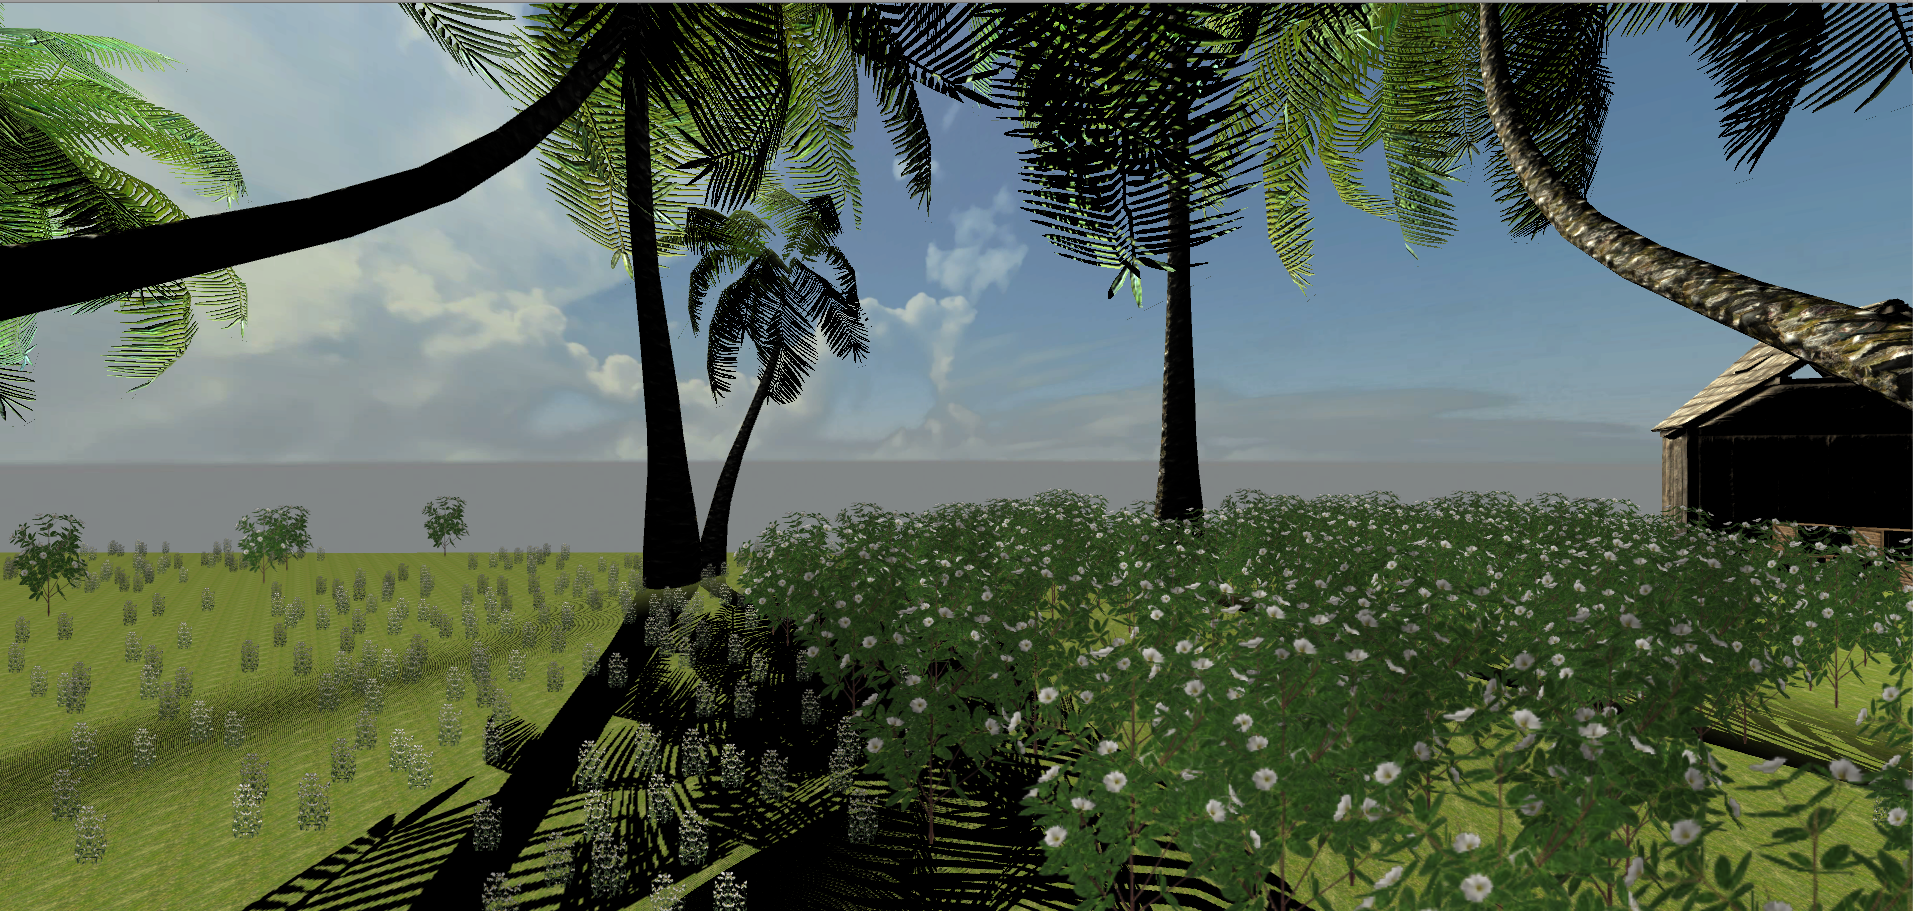
\includegraphics[width=0.235\textwidth]{Figures/island_reducedvision.png}
\label{fig:vision_range}}\\
\subfloat[]{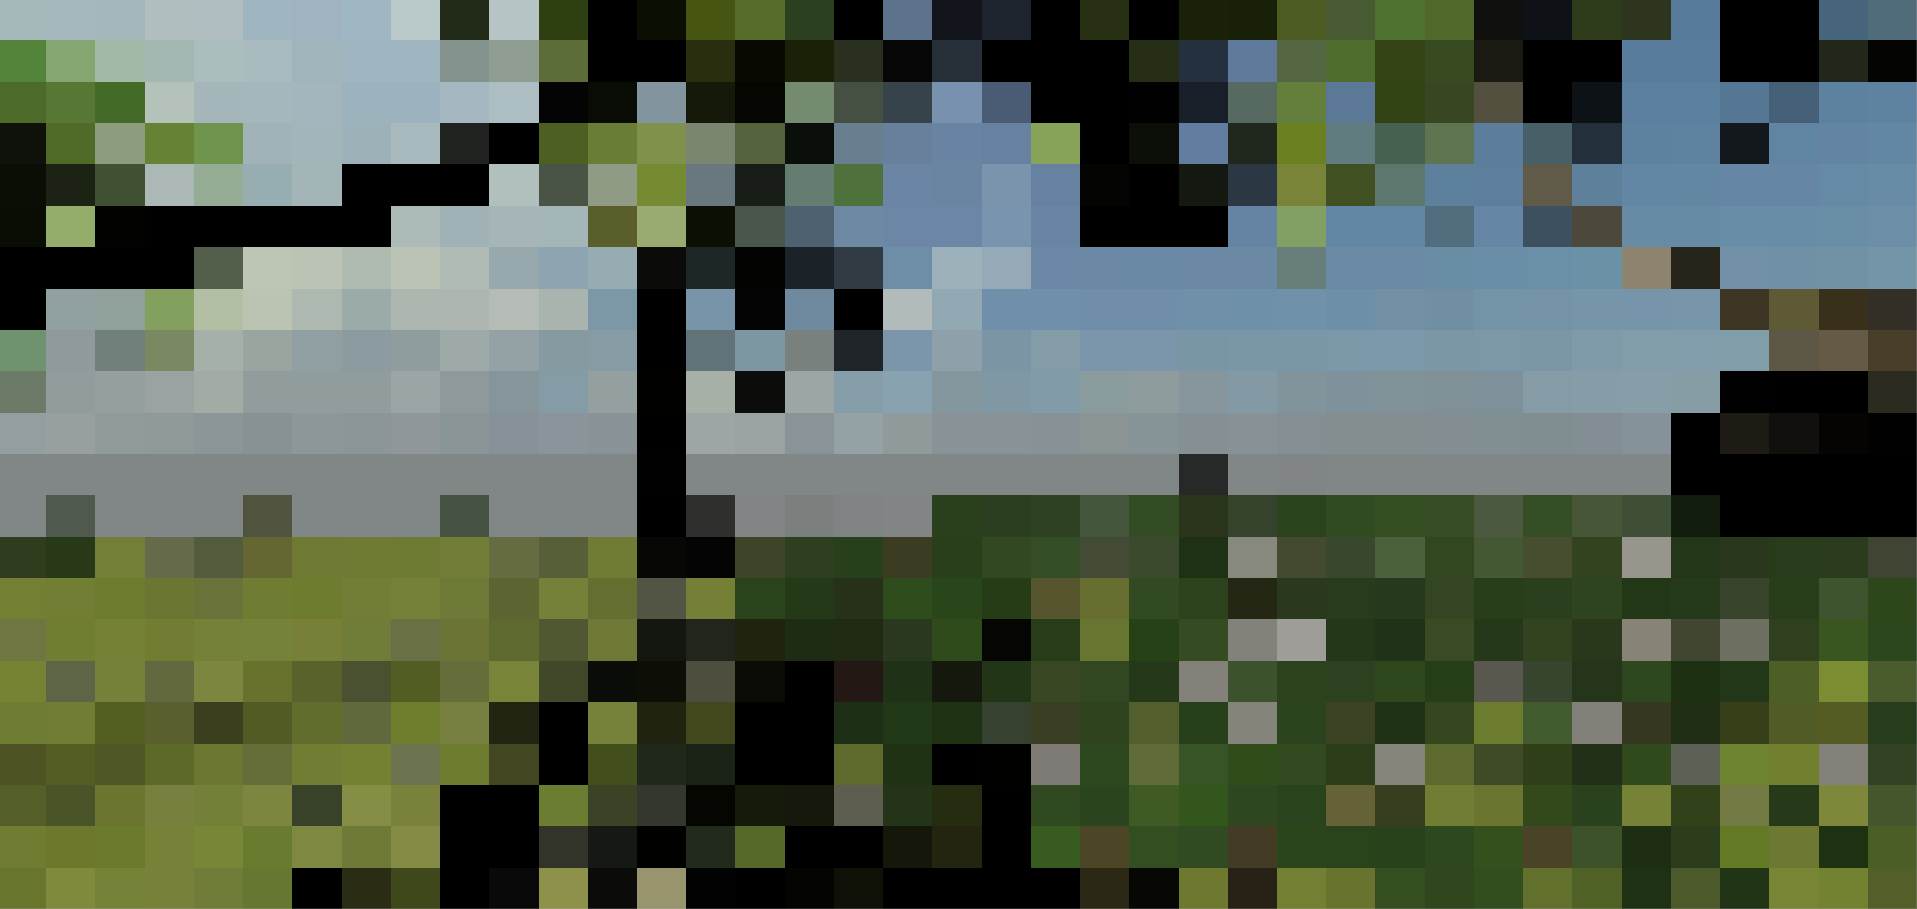
\includegraphics[width=0.235\textwidth]{Figures/island_reducedvision_highres.png}
	\label{fig:vision_highres}}
\subfloat[]{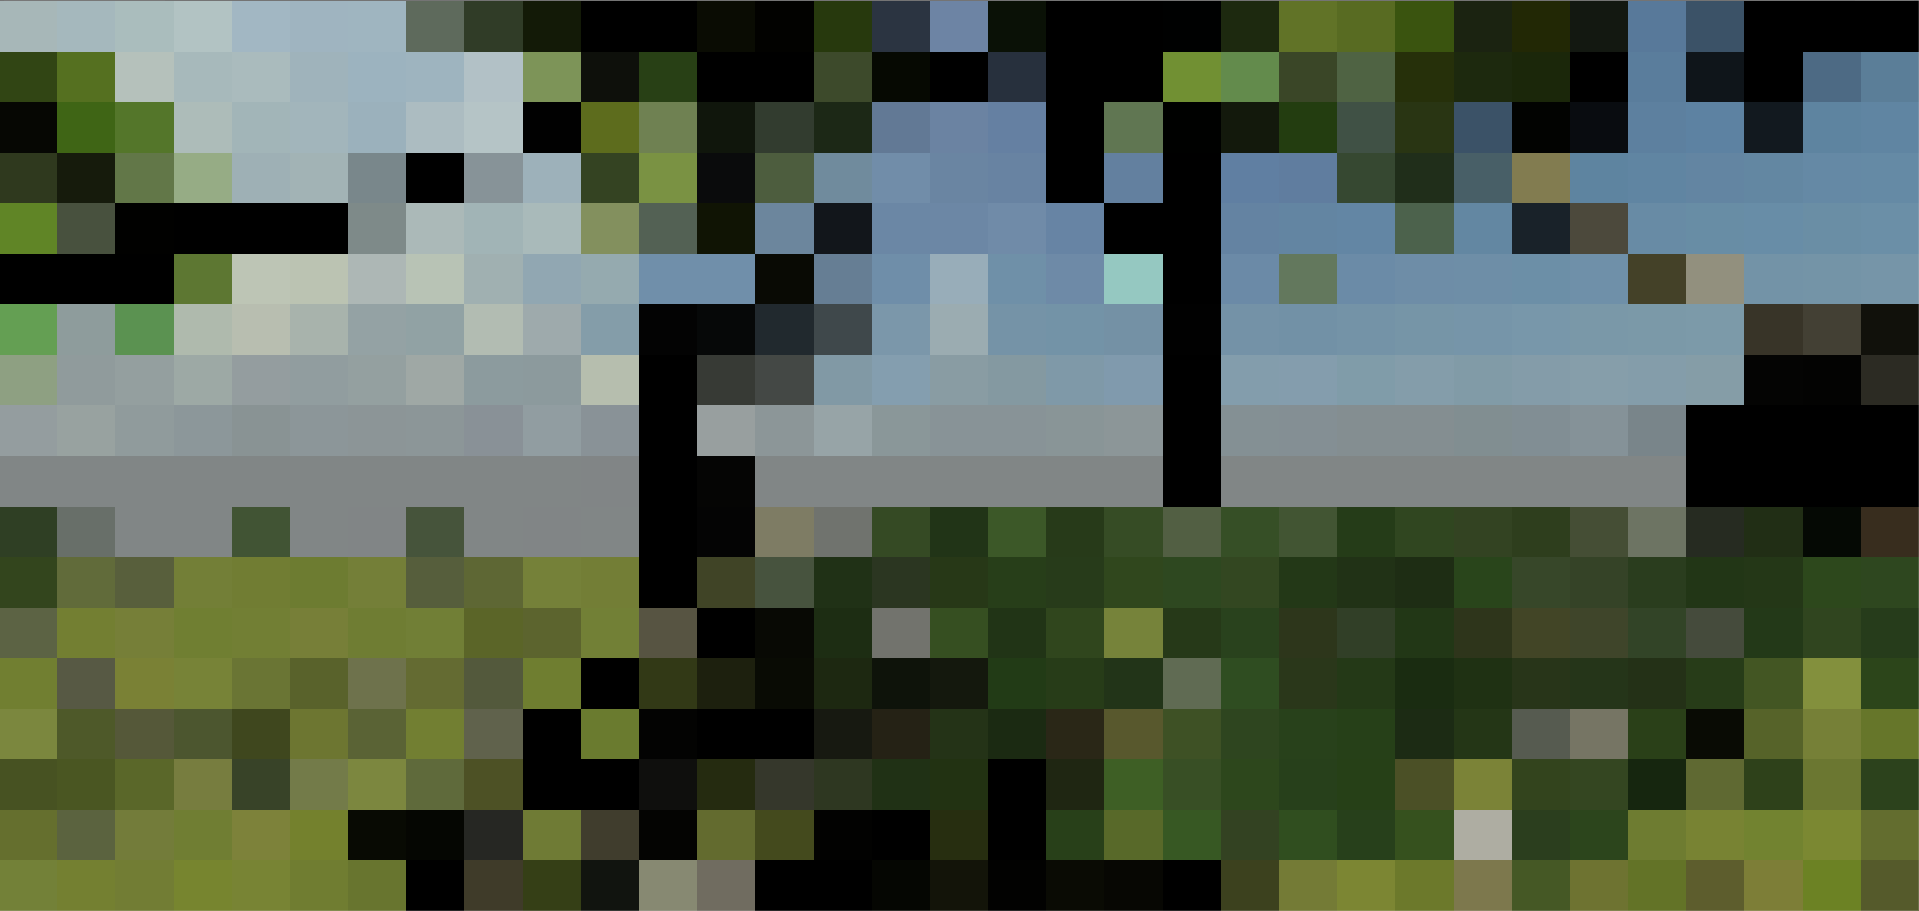
\includegraphics[width=0.235\textwidth]{Figures/island_reducedvision_lowres.png}
	\label{fig:vision_lowres}}

\caption{The same area of the simulation seen with different ``eyes'': (a) The simulation island without special, mosquito related processing of the picture (b) The range of vision has been reduced. (c) Reduced range of vision and reduced spatial resolution. (d) Reduced range of vision and stronger reduced spatial resolution.}
\label{fig:vision}
\end{figure}

\begin{figure}[ht!]
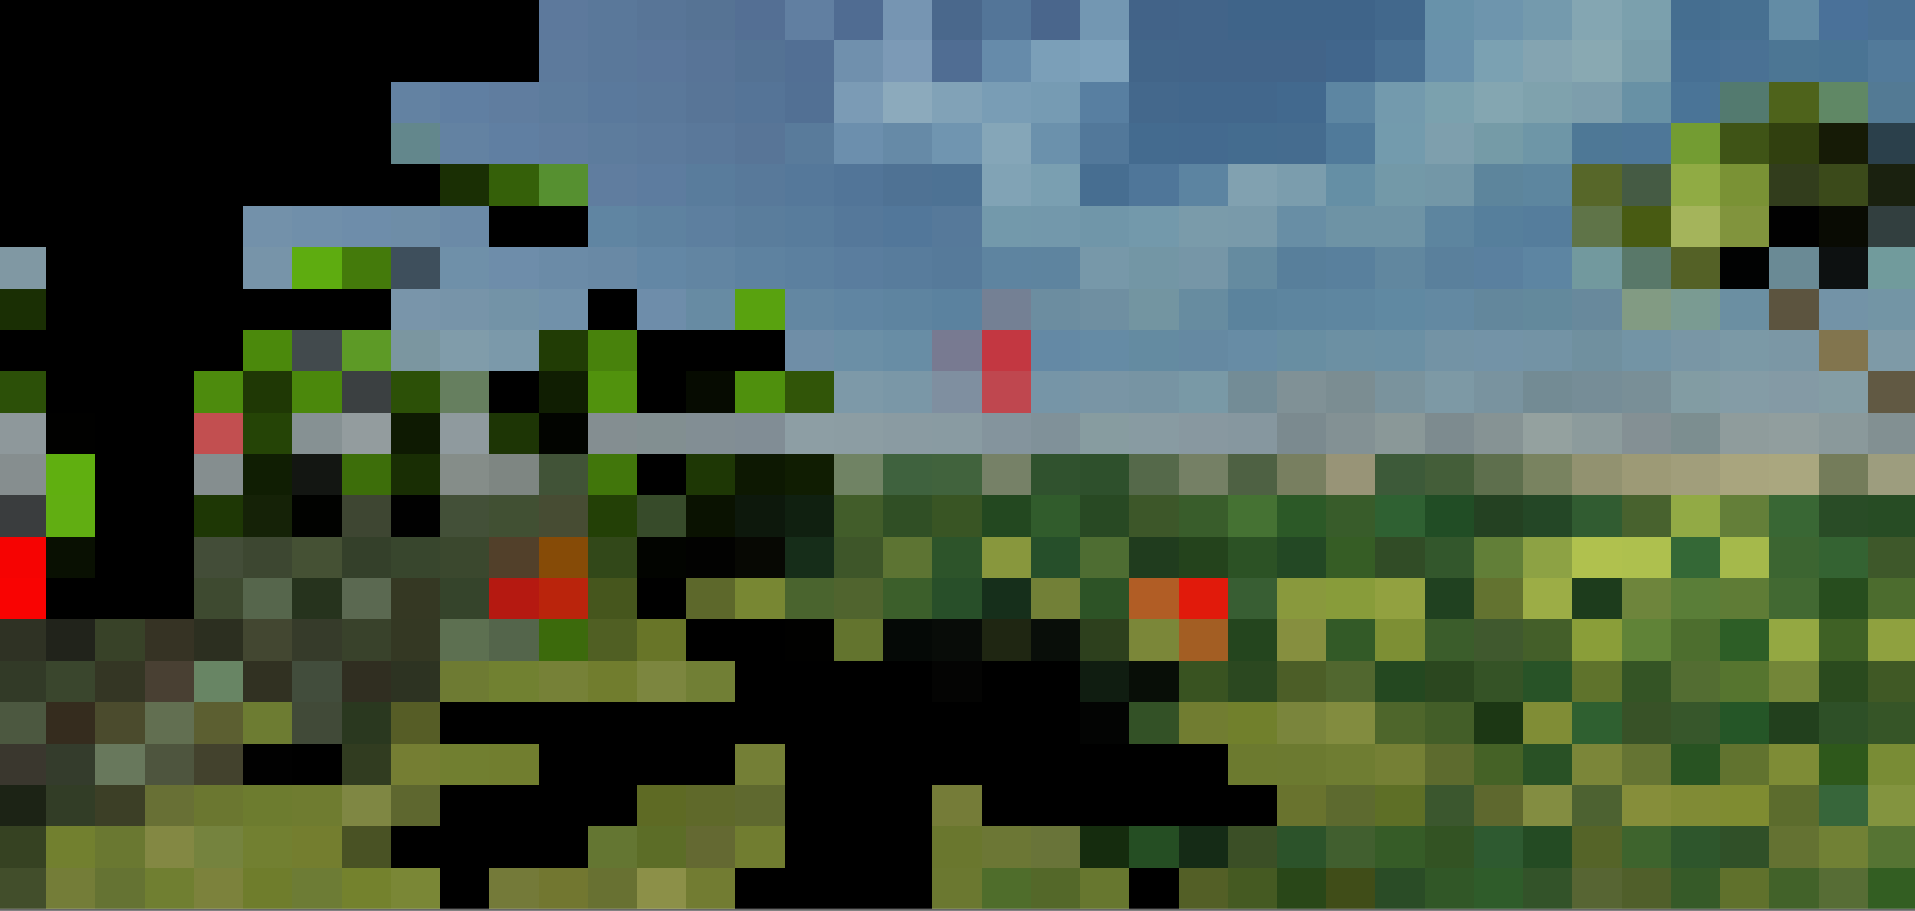
\includegraphics[width=0.47\textwidth]{Figures/co2.png}
\caption{Example for odour plumes (carbon-dioxide; red colour).}
\label{fig:co2}
\end{figure}
\vspace{3pt}

As soon as the user manages to follow these plumes to achieve a close enough proximity to see their prey, another important visual feature may become active. While compound eyes exhibit low spatial resolution, their temporal resolution is far higher. They excel in detecting motion. In the simulation we represent this with a flickering, yellow outline around moving animals (cf. Figure~\ref{fig:flickr}). The colour yellow was chosen, because of its uniqueness in the context of this simulation.

Last but not least, the heat sensors become active when the player manages to get very close to his prey. In this case, a special shader is activated, colouring the animal in a noticeable orange (cf. Figure~\ref{fig:heat}). This is especially important if the animal is sitting still, because without the colour it would be difficult to recognise the prey.


After the user has successfully tracked down a potential host and has managed to get close, he can land on the animal. As long as he is staying on the animal, he cannot move (but the animal can). He now may initiate the blood-sucking. Since mosquitoes represent an annoyance to every host when they feed on him, the prey may take counter measures. Screen shake and a vignetting effect (cf. Figure~\ref{fig:danger}) serve as tells for the player. In case the player decides to move away, he successfully fed on the hosts blood. If he fails to fly away in time, the simulation is over. After having fed successfully twice---irrespective of the difficulty level, the user has won and he will see a notification about the amount of points he acquired and a little high-score table. The amount of points he gathers, depend on the time it took the user to win. After that, the level starts all over with a higher difficulty. There are two difficulty levels. In the higher difficulty, the lower resolution (33x18) is used. Additionally, the movement speed of the mosquito is reduced by about 10\% and the range of vision is further reduced compared to the lower difficulty.

\begin{figure}[ht!]
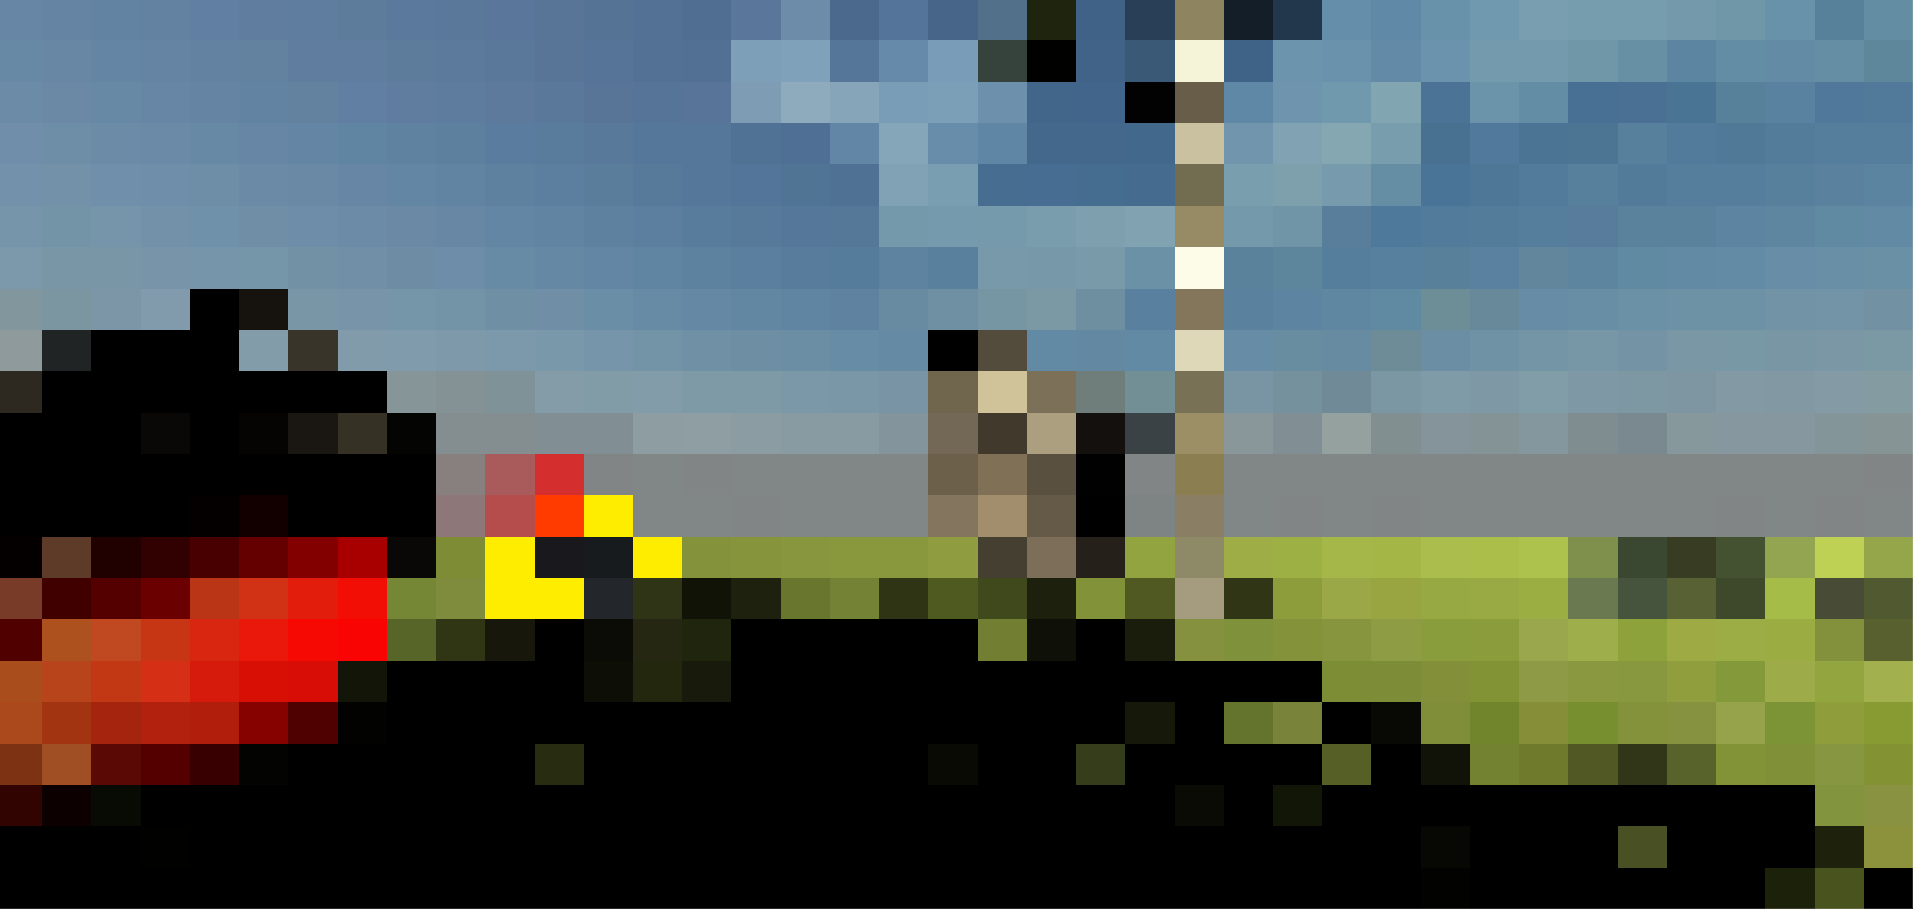
\includegraphics[width=0.47\textwidth]{Figures/flickr.png}
\caption{Flickering outline (yellow) induced by moving animals.}
\label{fig:flickr}
\end{figure}


\begin{figure}[ht!]
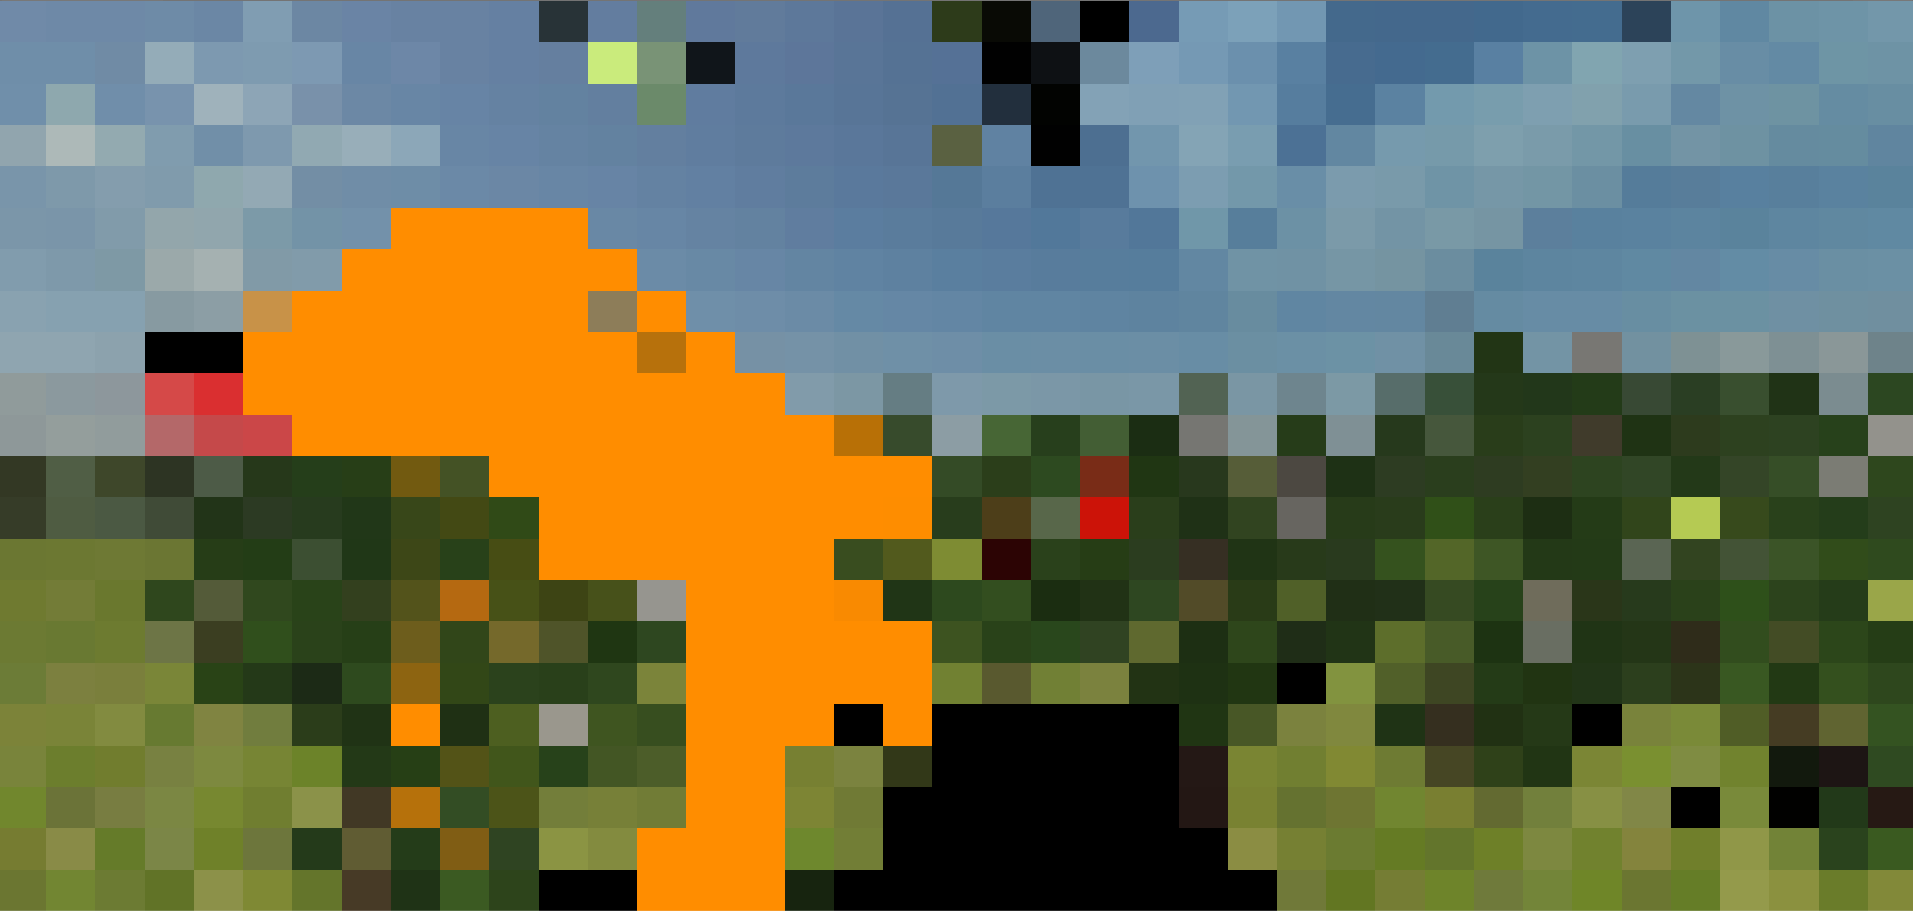
\includegraphics[width=0.47\textwidth]{Figures/heat.png}
\caption{Heat sensors signalling a nearby warm body (orange).}
\label{fig:heat}
\end{figure}



\begin{figure}[ht!]
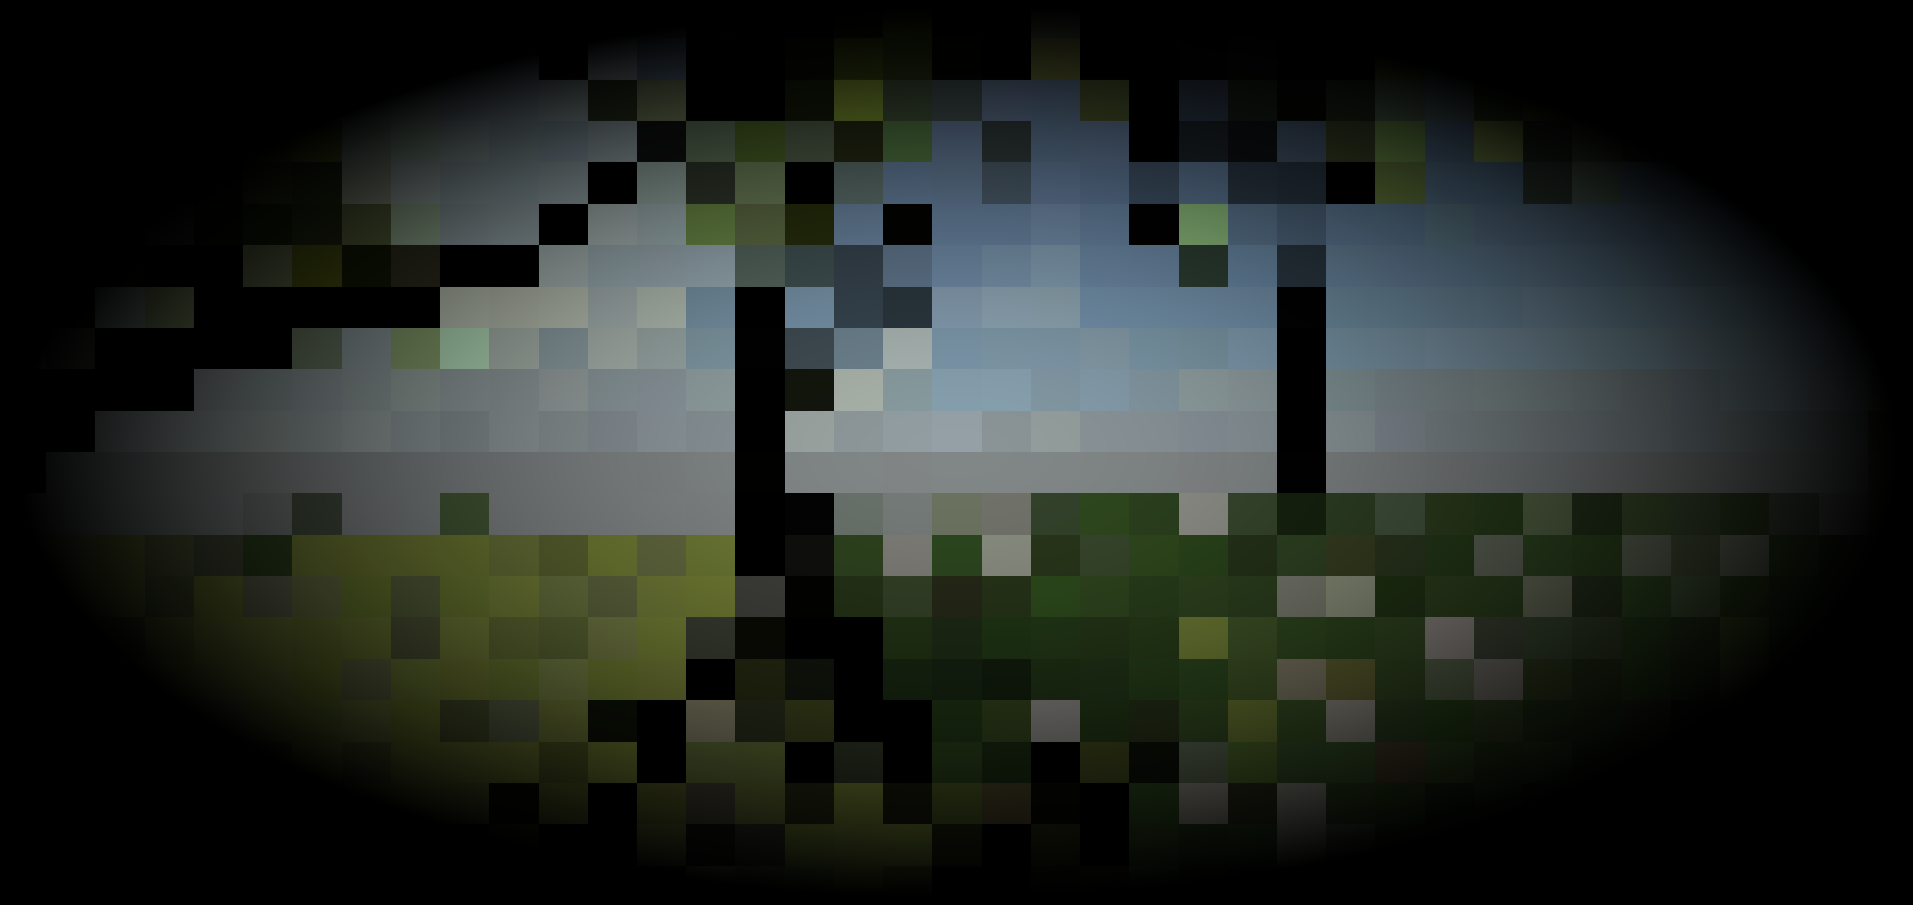
\includegraphics[width=0.47\textwidth]{Figures/danger.png}
\caption{During the process of blood sucking, the hosts may use counter measures. This is indicated to the player using screen shake and vignetting effects.}
\label{fig:danger}
\end{figure}



\subsection{User Experience}
\label{sec:ux}
The only help the player gets is the tutorial. It covers the key assignment, what the objective of the user is, and some screen shots explaining the game mechanics. Furthermore, during the simulation, there are neither button prompts nor any other UI. All information the user needs for his objective is conveyed in an immersive way, without any overlays inferring with the original, mosquito-inspired presentation. 
Due to the very alien nature of the picture presented to the user, it is difficult to recognise what he is actually looking at. This makes it necessary for the user to rely heavily on the given game mechanics (i.e. carbon-dioxide clouds, movement recognition, heat sensors) and learn how to use them. The carbon-dioxide plums, for example, will seldom directly lead to prey, because firstly, the prey could be moving, and secondly wind influences the movement direction of the plumes. It is up to the user to deduce the wind direction from observing the carbon-dioxide plumes.

\section{Project Requirements}
\label{sec:projectreq}

In this section, we will explain how scientific basics inspired the game mechanics in the interactive simulation (cf. Section~\ref{sec:proj_science}). In Section~\ref{sec:game}, we have a look at the user interaction and how these relate to gamifying the simulation. Afterwards, we discuss the learning tasks of the user (cf. Section~\ref{sec:complexity}) and, finally, in Section~\ref{sec:aesthetics}, we explain the driving motivations behind the realised aesthetics.

\subsection{Science}
\label{sec:proj_science}
The life circle of a mosquito has four phases: egg, larva, pupa, and adult~\cite{howstuff}. For our interactive simulation, we focus on the adult phase. As mentioned earlier, only female mosquitoes
feed on blood. For some species, this is mandatory in order to lay eggs, while for other species it increases the amount of eggs. The objectives, which a female mosquito aims to fulfil during its adult phase are: foraging, mating, blood sucking, and laying eggs. All these objectives can usually be repeated several times during the lifetime of a mosquito. For the purpose of this simulation, we focus on the perspective of a female mosquito, solely taking the aspect of feeding on blood into account.  

In our simulation we use carbon-dioxide representations in the form of red orbs (cf. Section~\ref{sec:senses}). Carbon-dioxide acts as an attractant for blood-seeking mosquitos. This is especially true when the mosquito senses $CO_2$ in the form of plumes in contrast to continuous occurrence. The distance mosquitoes can sense $CO_2$ is up to 35-50m~\cite{guerenstein2008, breugel2015}. Since this is farther than the mosquitoes ability to see, which seems to be around 5-15m~\cite{breugel2015}, it emphasises the importance of odour recognition for the mosquito's orientation. Furthermore, mosquitoes rather react to $CO_2$ in the form of plumes than to a continuous $CO_2$ occurrence~\cite{guerenstein2008}. Due to this importance, we decided to represent the $CO_2$ odours in our simulation in the described way. It resembles the facts regarding recognition distance, and plumes, and forces the user to rely on ``smelling'' until he has approached far enough. 
Furthermore, according to Breugel et al.~\cite{breugel2015}, mosquitoes become very active when sensing carbon-dioxide. We convey this in the simulation by increasing the movement speed of the mosquito for three seconds after he collided with $CO_2$.

As already mentioned, the range of vision of a mosquito is estimated to be 5-15m. This is taken into consideration in the scope of our simulation through reducing the camera's far clip plane.

\begin{figure}[h!]
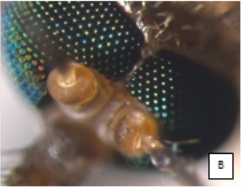
\includegraphics[width=0.47\textwidth]{Figures/compoundeye_real.png}
\caption{Compound eyes of a mosquito~\cite{singh2013}. The whole structure, as well as the individual ommatidia the compound eyes consist of, can be recognised. }
\label{fig:compoundeye_real}
\end{figure}

The compound eyes of mosquitoes consist of varying number of ommatidia. Singh~\cite{singh2013} counted the number of ommatidia for three species. According to him, the average number was between 610 and 900 ommatidia. We transferred this to a resolution of 33x18 respectively 39x22 in our simulation. Although the given number of ommatidia is counting only towards one compound eye, we stick with this number and, therefore, effectively only show a resolution that would be too low if we consider a normal mosquito with two compound eyes. However, the field of view of a mosquito is far greater than the 90 degree we used in the simulation. To compensate for this, staying with the resolution of one compound eye seems advisable.



In contrast to spatial resolution, compound eyes excel in temporal resolution~\cite{lehane2005}. This is expressed through the metric of \textit{flicker fusion frequency}(FFF) which ``is a function of the recovery time of the photoreceptors''. FFF in humans is between 20 and 30 flashes per second, while diurnal insects reach FFF values of around 200 to 300 Hz. In our simulation, this is integrated through drawing a flickering yellow outline around moving animals.

According to Breugel et al.~\cite{breugel2015} the heat sensors play an important role in the mosquito's decision where to land. This means this sensor information influences the behaviour only if the mosquito is very near to its prey. Furthermore, the heat sensors prevent the mosquito to land directly on the $CO_2$ source (e.g. the mouth of a human). In our simulation, we are colouring animals in a specific colour, when the user is very near to one. 


\subsection{Gamification}
\label{sec:game}
The user can control the mosquito in first person view. His objective is to follow the trail of carbon-dioxide plumes and visual indicators to approach a potential host. After landing on his prey, the user can initiate the feeding on blood. When the user recognises a screen shake and vignetting effect---this represents counter measures by the prey, e.g. trying to smash the mosquito (cf. Figure~\ref{fig:danger})---he must fly away from the animal in order to survive. All the interactions triggered by the user are done by pressing the right buttons. There are no button prompts or anything similar.

If the user manages to successfully feed on blood twice, he has won the round. After that he is prompted with the accumulated points. The number of points he earns is depending on the amount of time it took the user to achieve winning the round. 


\subsection{Complexity}
\label{sec:complexity}
The learning complexity of the user consists mainly of an adaptation process to the alien visual perception of the world. He has to learn not to rely on trying to identify any of the objects like, for example, trees or huts. Instead learning to follow the the plume orbs, inferring the wind direction, and anticipating the movement patterns of the animals are possible tasks he has to satisfy. Maintaining a sense of the spatial orientation will be another very difficult learning task. Due to the very limited range of vision in conjunction with the unfamiliar spatial resolution, it is vastly difficult for the user to know where he is.

\subsection{Aesthetics}
\label{sec:aesthetics}
The only GUI the simulation will offer is the main menu. This main menu is overlayed on top of the simulation and is rather transparent. Thus, the immersion is disturbed only to a very minor extend. The colours chosen for the fonts in the main menu are similar to the ones used for the main game mechanics (carbon-dioxide: red, movement detection: yellow, heat: orange). This means that both in the menu and in the simulation the important stuff has the same distinctly colours that differentiate themselves very well from the rest.
Besides the main menu no GUI exists. Controlling the mosquito requires the user to memorize a few key assignments, which he can find in the tutorial.

The island itself consists of realistic modelled objects. Due to the way we impair the vision in order to approximate a mosquito's perception, it results in a very strong pixel look. This makes it difficult, but not impossible, to recognize the objects in the simulation world. We adjusted the size of the world specifically in a way that conveys the smallness of a mosquito, while still enabling the user to successfully guess what he is seeing.

The used colours of the island are mostly blackish, brownish and greenish. Particularly, the used colours for the game mechanics (carbon-dioxide: red, movement detection: yellow, heat: orange) are very distinct from the rest. This distinction serves to roles. Firstly, the aforementioned colours are no real physical objects in the world. All three are representations for senses. This means visual information that would not be available in the real world is separated through colours from the rest of the simulation word. Secondly, these colours are very easy to identify for the user. They can be seen as signal colours. Thus, this makes it naturally possible for the user to easily distinguish important information for the hunt for blood from unimportant information. 


\section{Summary \& Future Work}
\label{sec:summary}

In this paper we presented an interactive simulation, where the user controls a mosquito. Thereby, we focussed on the process of feeding on blood. The simulation is set on a tropical island. The users objective is to search for prey in order to get some blood. In order to achieve this, he is offered an appropriate mapping of relevant mosquito senses to the simulation. Depending on the distance to his prey, the user can either rely on following a trail of carbon-dioxide, recognising movement and approaching it, or recognising heat sources. While feeding on blood, the user has to be aware of the host's counter measures. After having successfully reacted to the hosts defences, the user's feeding on blood was fruitful. If he manages to feed on blood twice, he wins and can start a new simulation on a higher difficulty level.


The current state of the simulation is a proof-of-concept. We suggest several extensions for the future. 
The two main suggestions are related to the perceived colours and field of view. The spectral sensitivity of mosquitoes ranges from 323nm (ultraviolet) to 621nm (orange-red)~\cite{muir1992}. This means that mosquitoes cannot sense red, but can sense ultraviolet. In order to cut the red from the picture, we propose firstly make some imaging using filter which suppress red. After that it would be possible to deduce how to manipulate the images in the simulation to achieve a similar effect. The same could be done for ultraviolet. Additionally, one could extend the simulation with a game mechanic for finding food in the form of flowers. Flowers shows unique shapes and signs when only their ultraviolet emission is viewed. This information is used by insects to determining the type of flower and the precise location of nectar.

The second suggestions concerns the field of view. Compound eyes supply their hosts with a far wider field of view than what we use in the simulation. To represent this in the simulation, we propose to use a pannini projection~\cite{sharpless2010}. This is a very good projection to receive rectangular images (like on a monitor), while not displaying strong distortions (cf. Figure~ref{fig:pannini}). Therefore, we could, for example, use a camera rig of five cameras (front, left, right, top, bottom) and project their images in form of a render to some meshes forming a fish-eye. Afterwards, we can calculate the pannini projection on a rectangle.

\begin{figure}[ht!]
 %   \centering
\subfloat[]{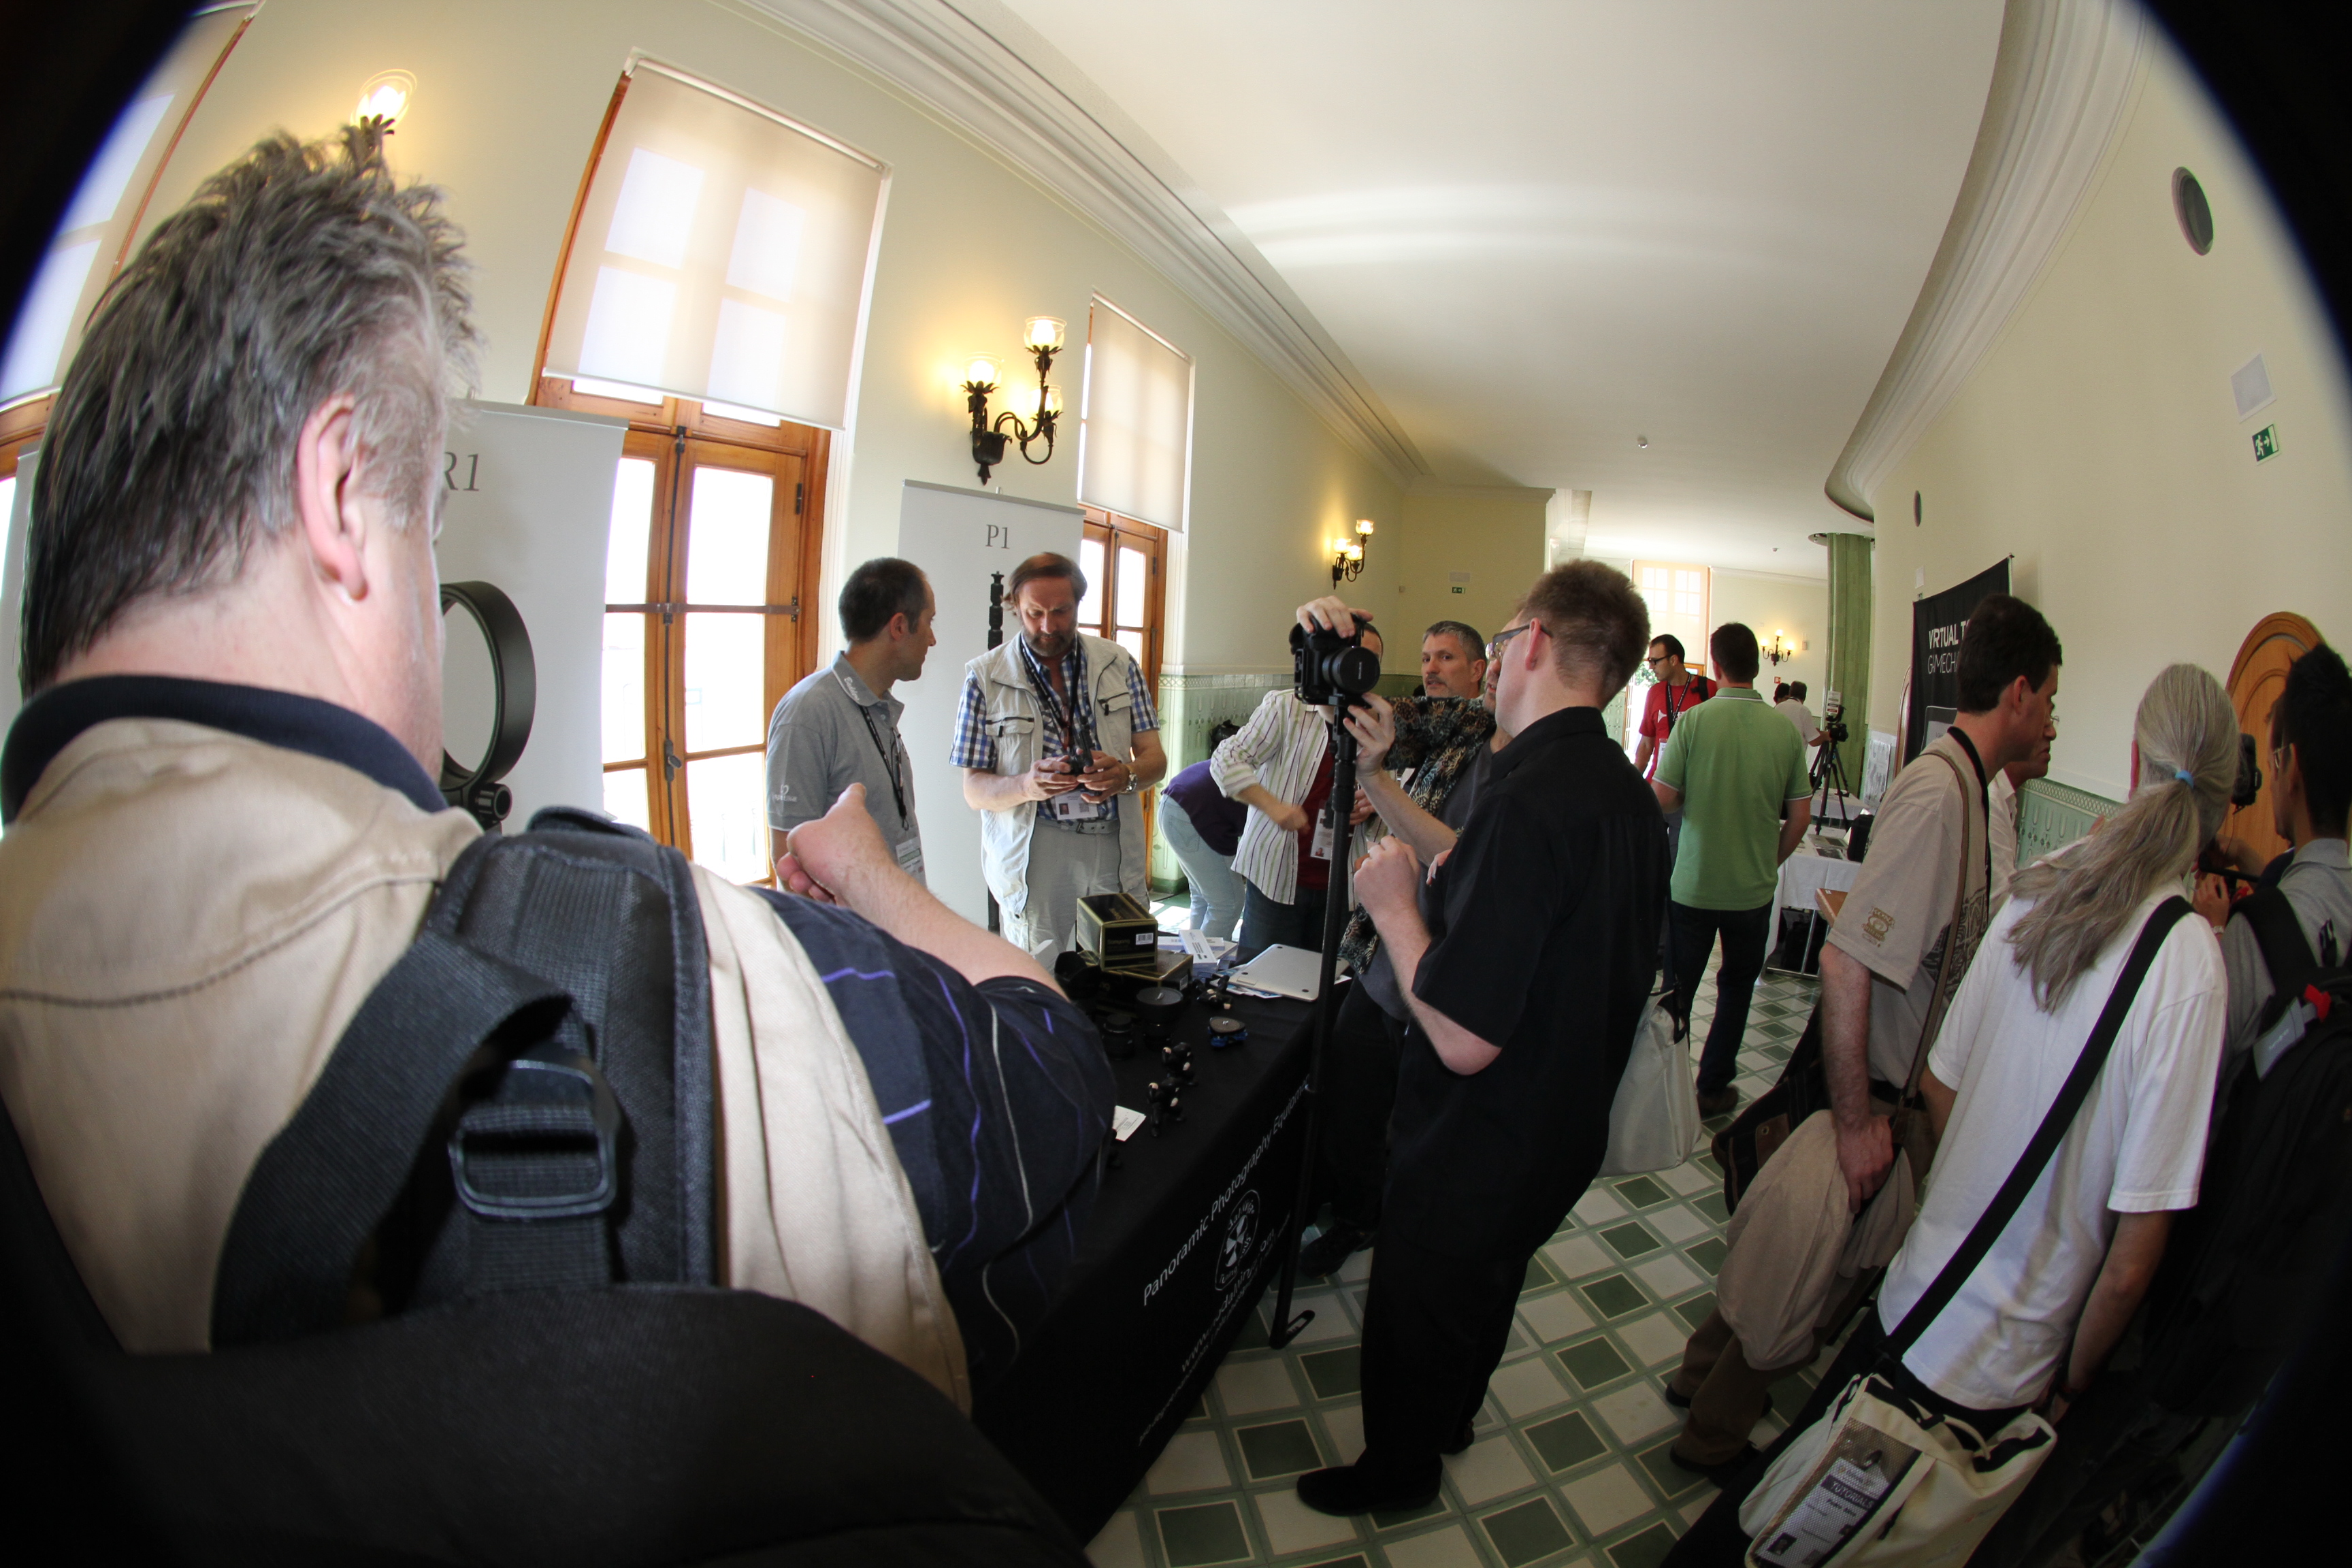
\includegraphics[width=0.235\textwidth, height=3cm]{Figures/Panini_fisheye.jpg}
	\label{fig:fisheye}}
\subfloat[]{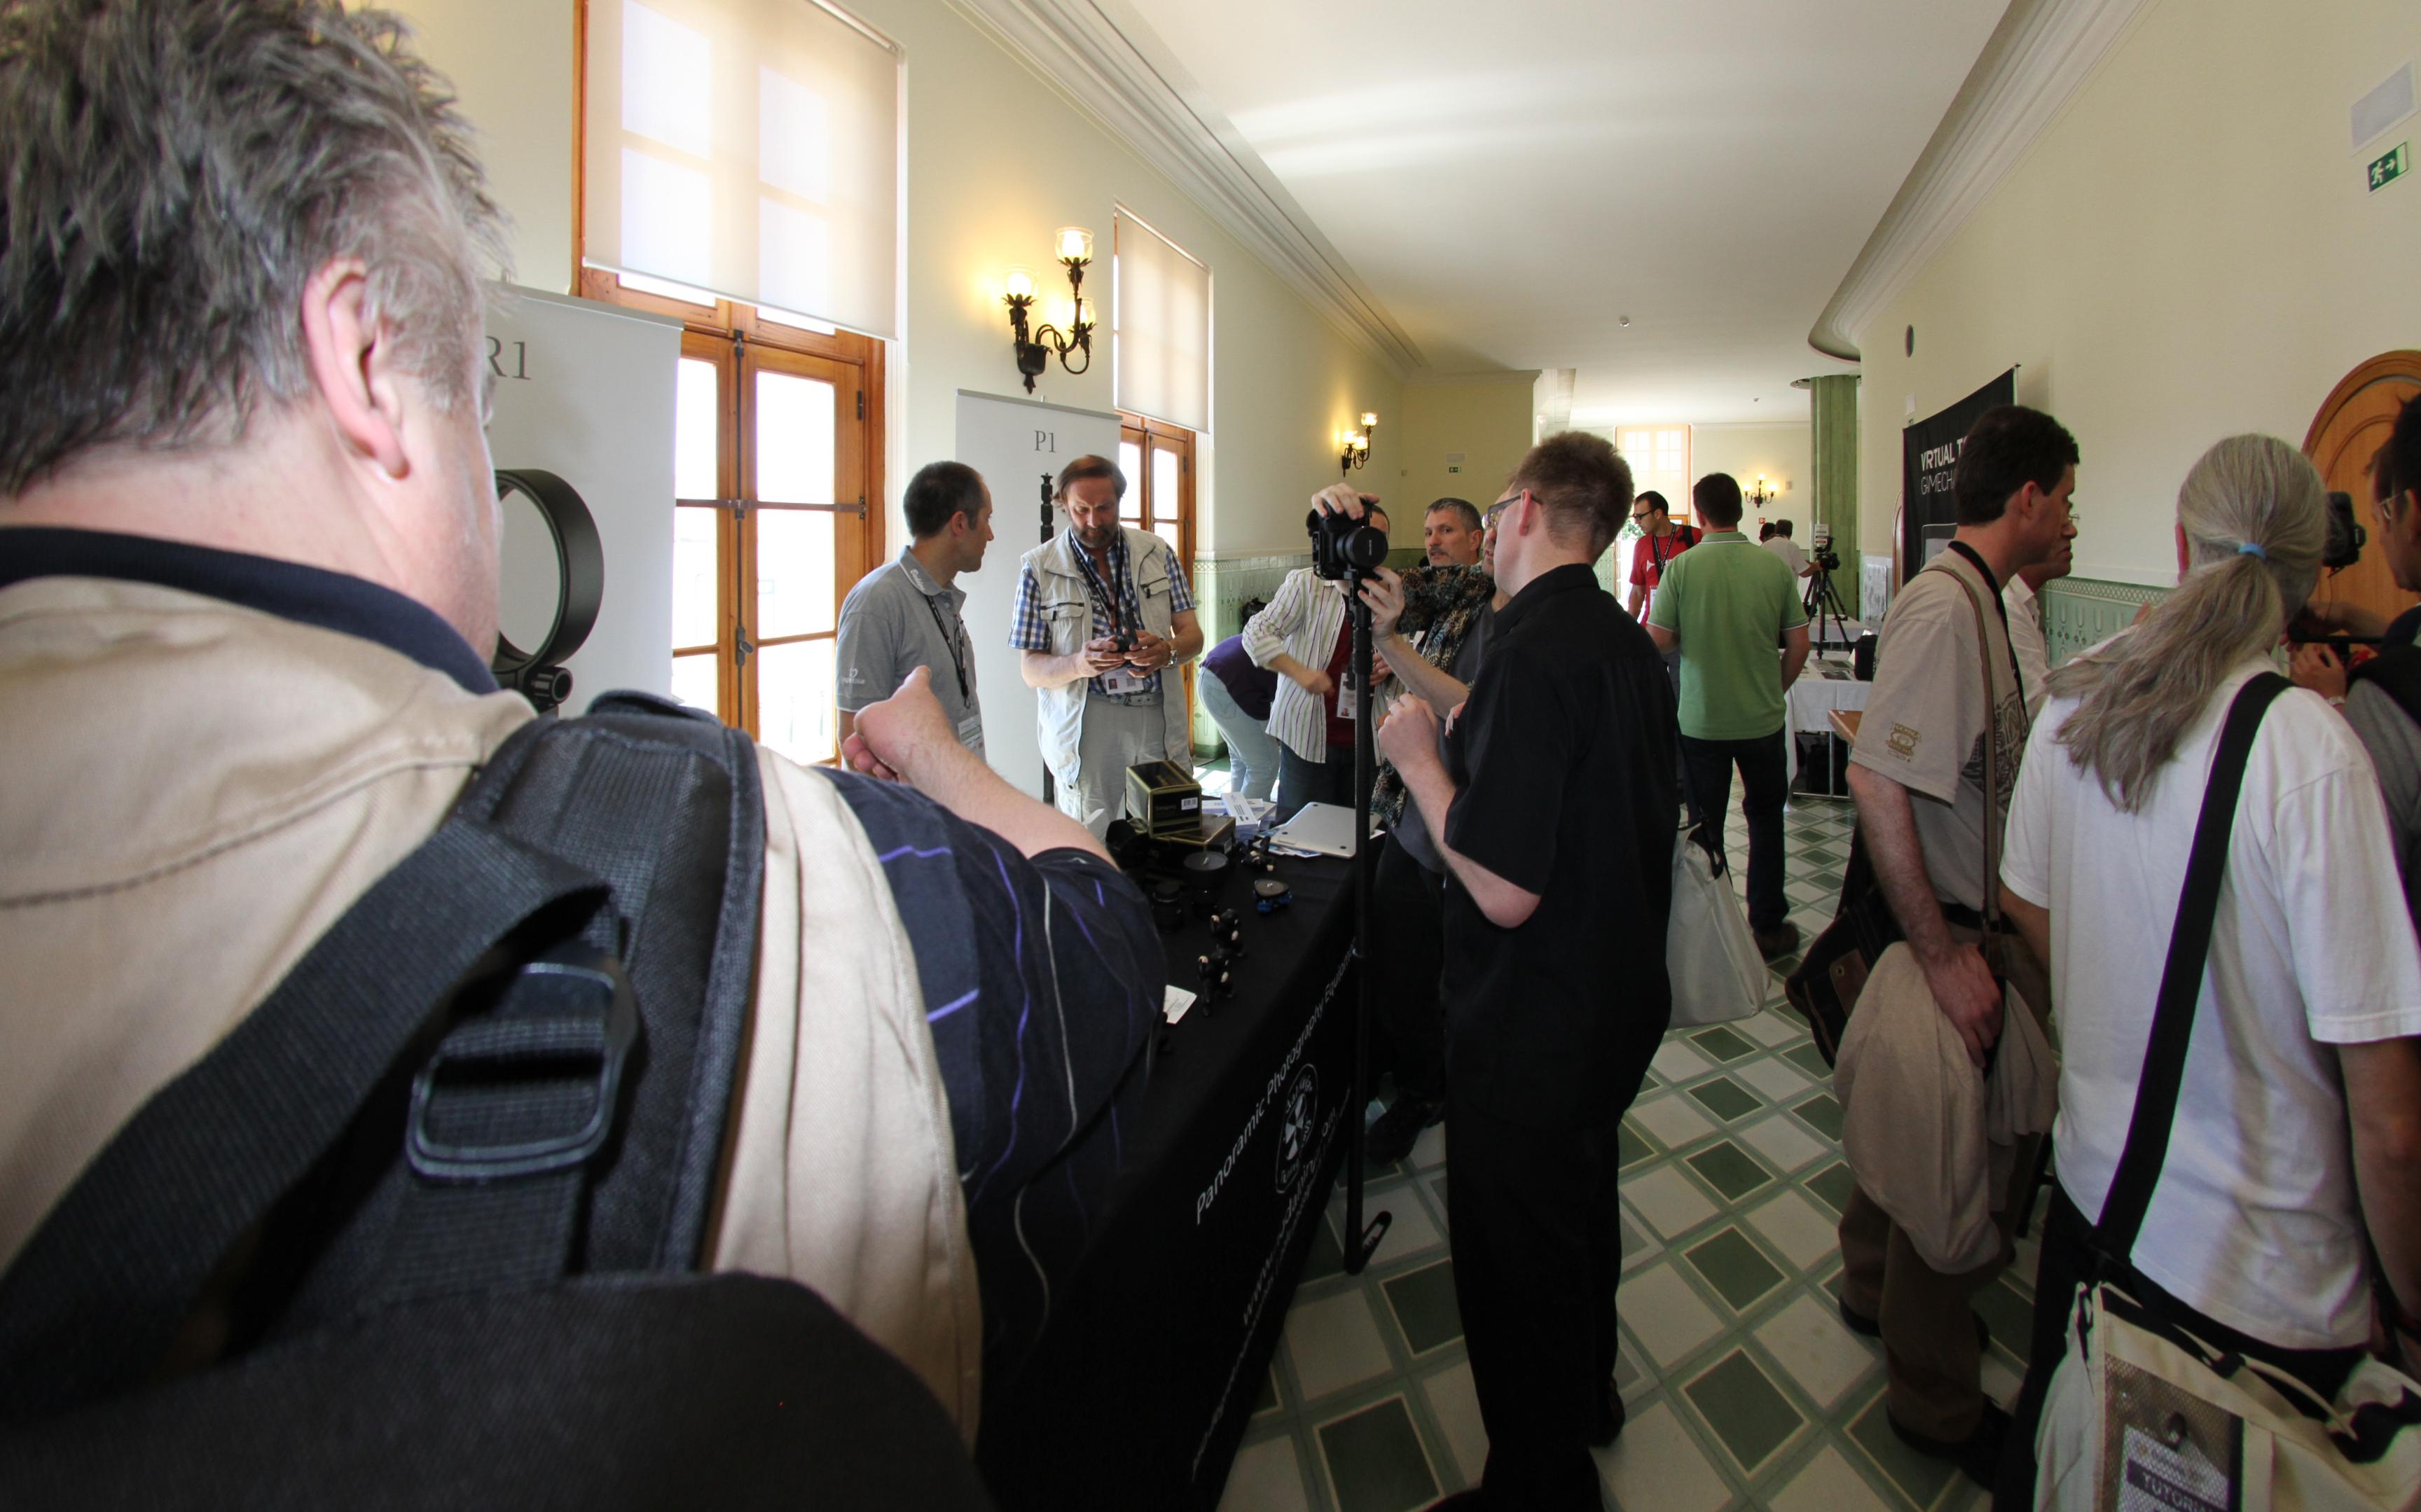
\includegraphics[width=0.235\textwidth, height=3cm]{Figures/Panini_nofisheye.jpg}
\label{fig:fish_pannini}}

\caption{Figure (a) shows s fish-eye photo with clear distortion. (b) The same picture after image processing with a pannini projection was applied.}
\label{fig:pannini}
\end{figure}


%According to Breugel et al.~\cite{breugel2015} mosquitoes become very active when sensing carbon-dioxide. Increasing the movement speed of the mosquito in the simulation would be a nice little implementation of this detail.

Furthermore, a more realistic movement detection is advisable. The flicker effect of moving animals should only be visible when the animal is moving more or less orthogonal to the viewing direction of the mosquito. In addition, the flicker should only be visible if the surrounding's contrast relative to the animal texture is greater than a specific threshold.

Last but not least, creating a better model of the compound eye, using different ommatidia densities for different eye regions would be necessary to reasonably present the world through compound eyes. A starting point may be the work of Neumann~\cite{neumann2002}, where he describes an algorithm that reconstructs the field of view of compound eyes.


\bibliographystyle{ieeetr}
\bibliography{sciwri}  

\end{document}
